%\modeCorrection


\renewcommand{\thesubsection}{\textcolor{red}{\Roman{section}.\arabic{subsection}}}
\renewcommand{\thesubsubsection}{\textcolor{red}{\Roman{section}.\arabic{subsection}.\alph{subsubsection}}}
\renewcommand{\titreDocu}[1]{
  \refstepcounter{document} % update counter
  \textbf{Exercice \arabic{document} -- #1} 
  \addcontentsline{toc}{document}{\protect\numberline{} #1} % update table of content
}

\setcounter{section}{0}
\setcounter{document}{0}


\nomPrenomClasse
\vspace{1cm}

\begin{center}
\begin{mdframed}[style=titr, leftmargin=60pt, rightmargin=60pt, innertopmargin=7pt, innerbottommargin=7pt, innerrightmargin=8pt, innerleftmargin=8pt]
\begin{center}
\begin{Large}
    Devoir Surveillé n°3 (sujet B) : Propagation de la lumière dans les milieux (55min)
\end{Large}
\end{center}
\end{mdframed}
\end{center}
\vspace{1cm}

\begin{tableauCompetences}
    APP & Connaître les définitions du cours & & & & \\
    \hline
    REA & Réaliser ou compléter un schéma & & & & \\
\hline
    ANA &  Exploiter des informations extraites des données & & & & 
\end{tableauCompetences}

\begin{tcolorbox}[colback=red!5!white,colframe=red!75!black,title=\textbf{Consignes : }]
   \begin{enumerate}
        \item Vous rédigerez tout sur le sujet,
        \item Pour les élèves bénéficiant d'un PAP, vous ne traiterez pas les questions marquées par $(*)$ ; 
        %\item La calculatrice \underline{n'est pas autorisée}.
   \end{enumerate}
\end{tcolorbox}

\begin{doc}{Quizz \begin{Large}
    /4 points
\end{Large}}
Entourer \underline{la} bonne réponse :
\begin{enumerate}
    \item \textbf{L'indice optique d'un milieu est (1pt):}
        \begin{align*}
            a.& ~\text{plus petit que 1} & b.& ~\text{plus grand que 1} & c.& ~\text{égal à 1 dans le plexiglas} 
            %a.& ~\text{plus petit que 1} & b.& ~\text{\textcolor{red}{plus grand que 1}} & c.& ~\text{égal à 1 dans le plexiglas} 
        \end{align*}
    \item \textbf{$(*)$Une normale au dioptre est (1pt):}
        \begin{align*}
            a.& ~\text{un objet qui permet de disperser la lumière} & b.&~\text{une ligne imaginaire perpendiculaire à l'interface} \\
            c.& ~\text{l'interface entre deux milieux différents} & d.&~\text{un instrument de musique}
            %a.& ~\text{un objet qui permet de disperser la lumière} & b.&~\text{\textcolor{red}{une ligne imaginaire perpendiculaire à l'interface}} \\
            %c.& ~\text{l'interface entre deux milieux différents} & d.&~\text{un instrument de musique}
        \end{align*}
    %\item (*)\textbf{Un rayon lumineux passant par la normale (1pt): }
    %    \begin{align*}
    %        a.& ~\text{le rayon n'est pas dévié à l'interface} & b.& ~\text{il y a réfraction à l'interface} \\
    %        c.& ~\text{Le rayon s'éloigne de la normale} & d.& ~\text{le rayon se rapproche de la normale}
            %a.& ~\text{le rayon n'est pas dévié à l'interface} & b.& ~\text{\textcolor{red}{il y a réfraction à l'interface} } \\
            %c.& ~\text{Le rayon s'éloigne de la normale} & d.& ~\text{\textcolor{red}{le rayon se rapproche de la normale}} 
    %    \end{align*}
    \item \textbf{La lumière se propage dans le vide à la vitesse (1pt):}
        \begin{align*}
            a.& ~\text{$c=3\times10^8$~km$\cdot$h$^{-1}$} & b.& ~\text{$c=3\times10^8$~m$\cdot$s$^{-1}$} & c.& ~\text{$c=340$~m$\cdot$s$^{-1}$ à la température T=15$\degreCelsius$}
            %a.& ~\text{$c=3\times10^8$~km$\cdot$h$^{-1}$} & b.& ~\text{\textcolor{red}{$c=3\times10^8$~m$\cdot$s$^{-1}$}} & c.& ~\text{$c=340$~m$\cdot$s$^{-1}$ à la température T=15$\degreCelsius$}
        \end{align*}
    \item \textbf{La rétine de l'\oe il (1pt):}
    \begin{align*}
            a.& ~\text{se modélise par une lentille convergente} & b.~\text{est fait en cristal} \\
            c.& ~\text{convertit un signal lumineux en signal électrique} 
            %a.& ~\text{se modélise par une lentille convergente} & b.& ~\text{est fait en cristal} \\
            %c.& ~\text{\textcolor{red}{convertit un signal lumineux en signal électrique}} 
        \end{align*}
\end{enumerate}
\end{doc}

\begin{doc}{L'objectif d'un microscope \begin{Large}
    /8 points
\end{Large}}
%\begin{wrapfigure}{r}{0.2\textwidth}
\begin{center}
    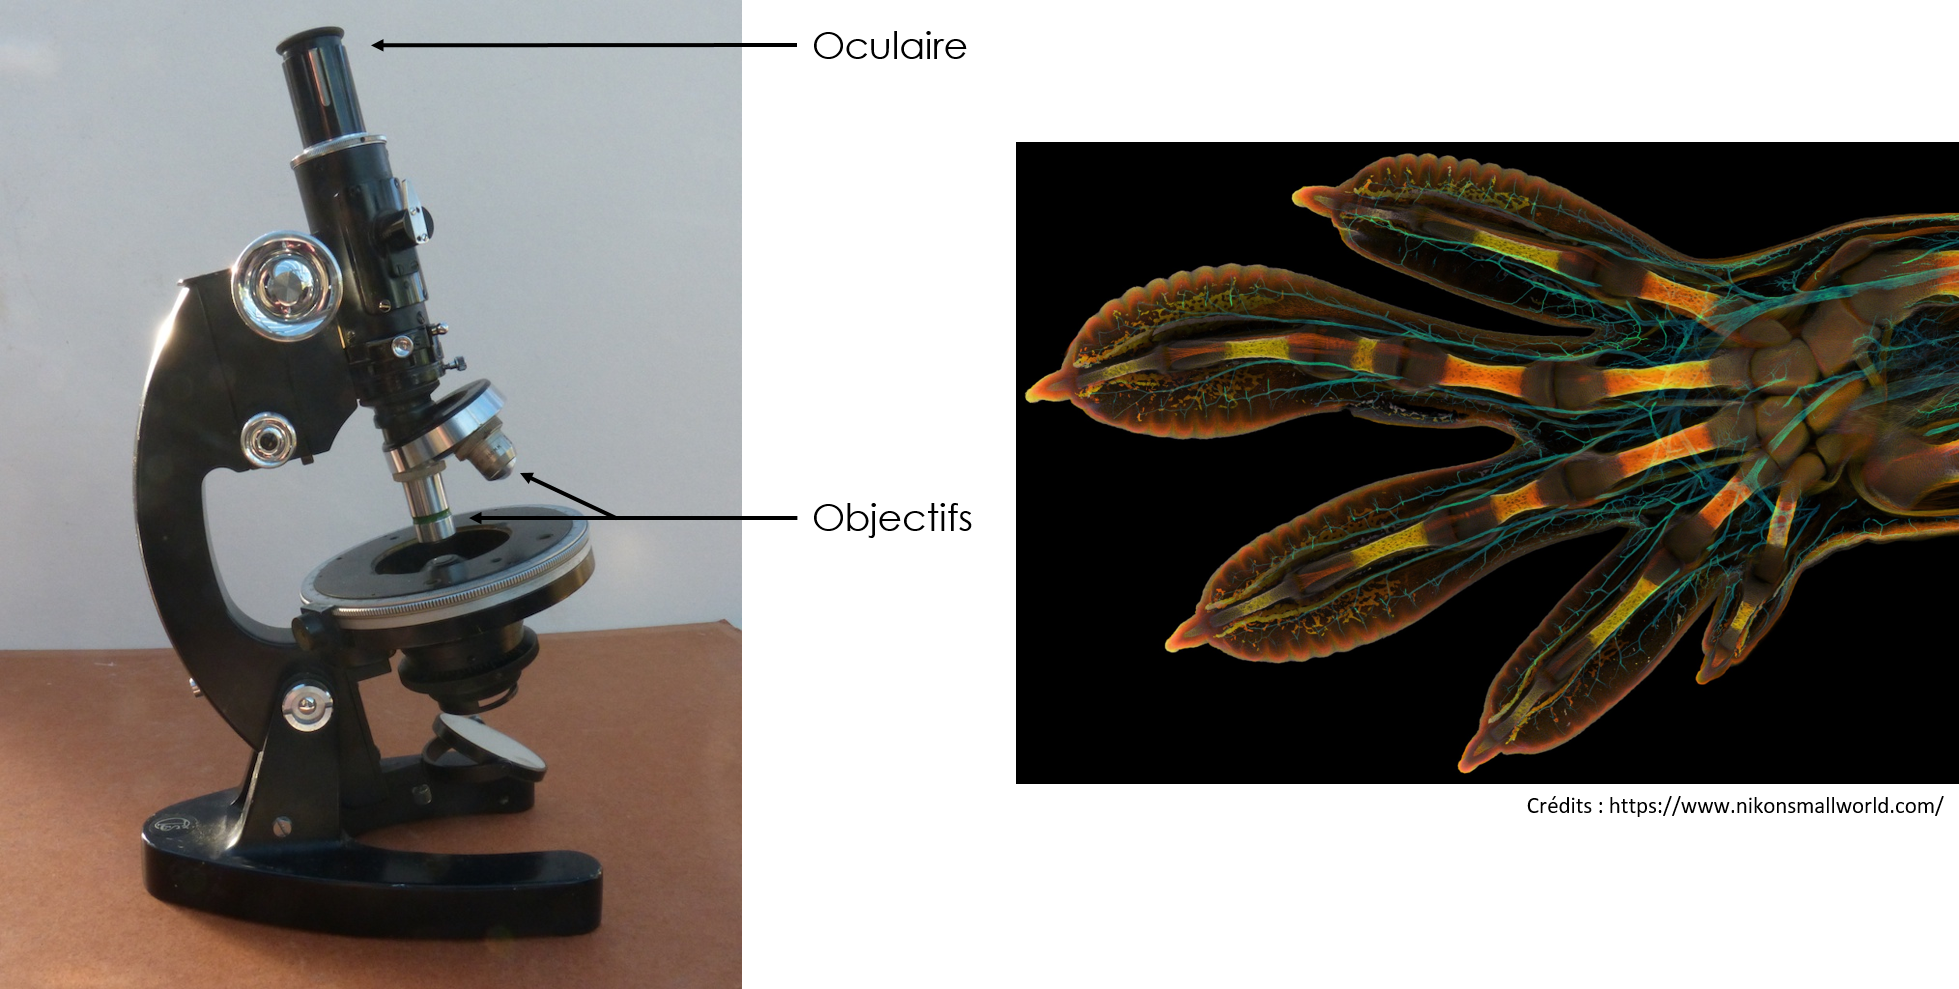
\includegraphics[scale=0.4]{Images/Microscope.png}
\end{center}
      
 % \end{wrapfigure}
L'image de droite ci-dessus représente l'image d'une patte de Gecko embryonnaire obtenue à l'aide d'une technique de microscopie très particulière appelée \og confocale \fg. Cette image a remporté le prestigieux concours d'imagerie de microscopie en 2022 organisé chaque année par la marque Nikon.\\
Un microscope sert à rendre visible pour l'\oe il des objets de taille microscopique (jusqu'au dixième de nanomètre pour les meilleurs microscopes !). \\
Un microscope standard est constitué d'un oculaire et d'un ou de plusieurs objectifs (voir la figure de gauche ci-dessus) qui sont tous les deux des lentilles convergentes. On se propose ici d'évaluer le grandissement d'une lentille convergente.

\question{Compléter le schéma ci-dessous avec les informations suivantes : centre optique \textbf{O}, \textbf{axe optique}, foyer focal objet \textbf{F}, foyer focal image \textbf{F'}. (2pts)
\begin{center}
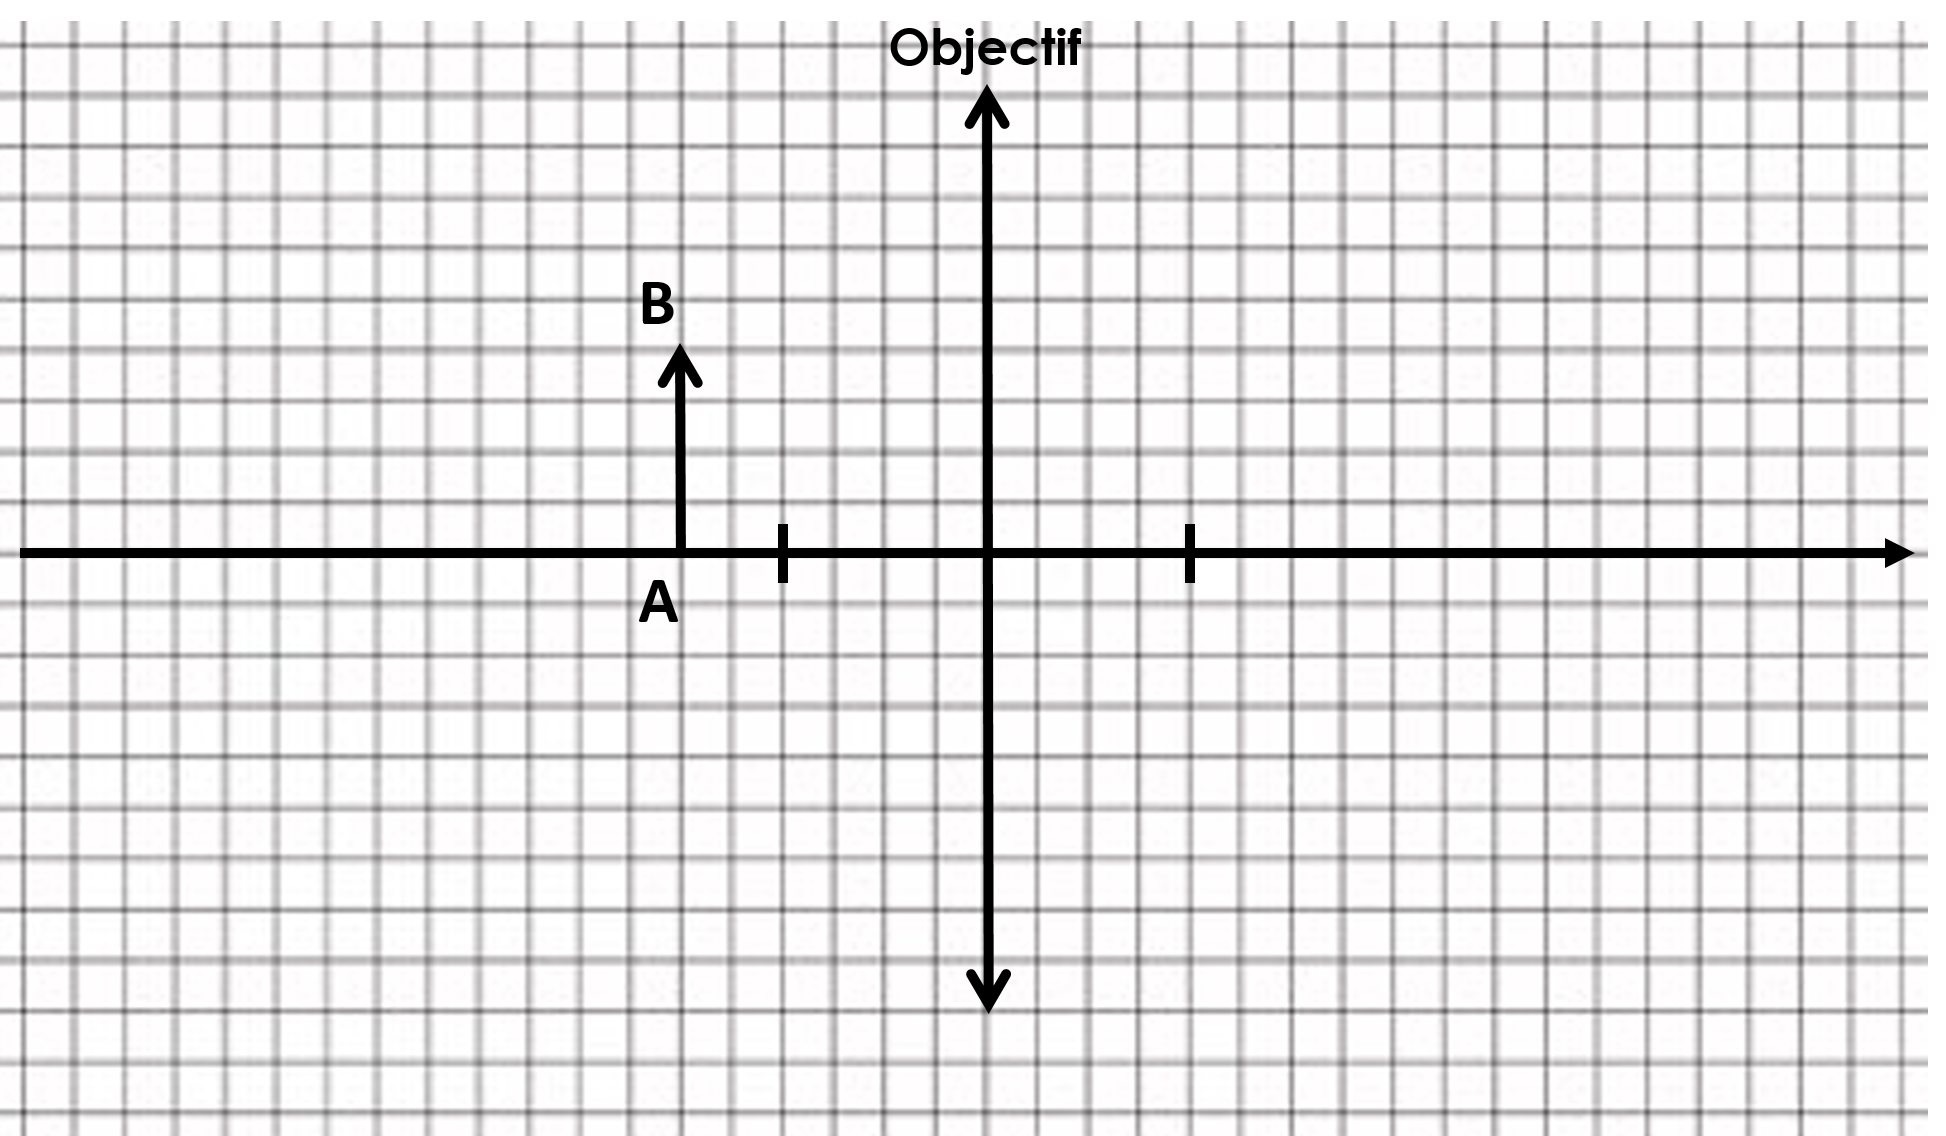
\includegraphics[scale=0.45]{Images/Construction_lentille_SujetB.png}    
\end{center}}{\begin{center}
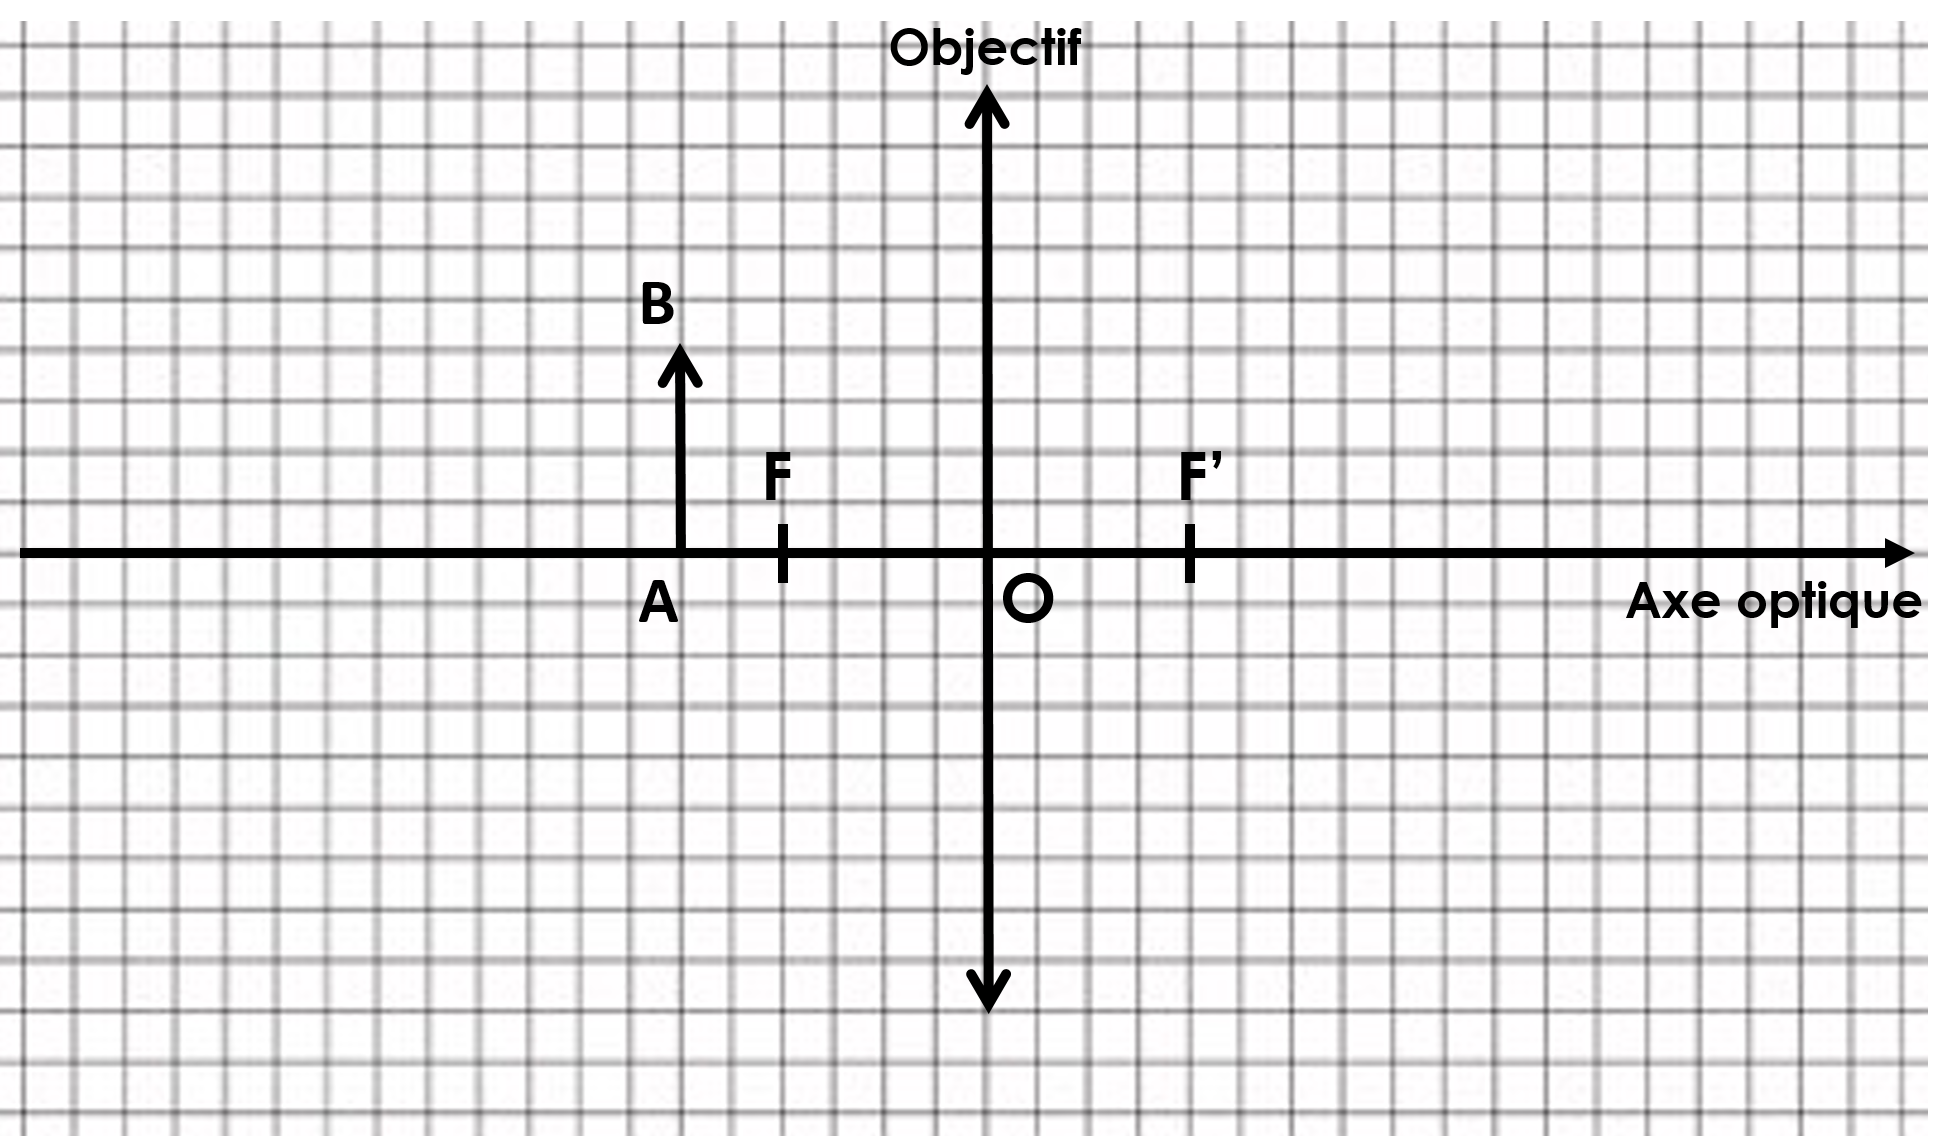
\includegraphics[scale=0.45]{Images/Construction_lentille_SujetB_correction1.png}    
\end{center}}{0}
%\\
%\vspace{-5pt}
\question{\`{A} l'aide d'au moins deux rayons lumineux, construire sur le schéma précédent l'image A'B' de AB à travers la lentille. (2pts)}{\begin{center}
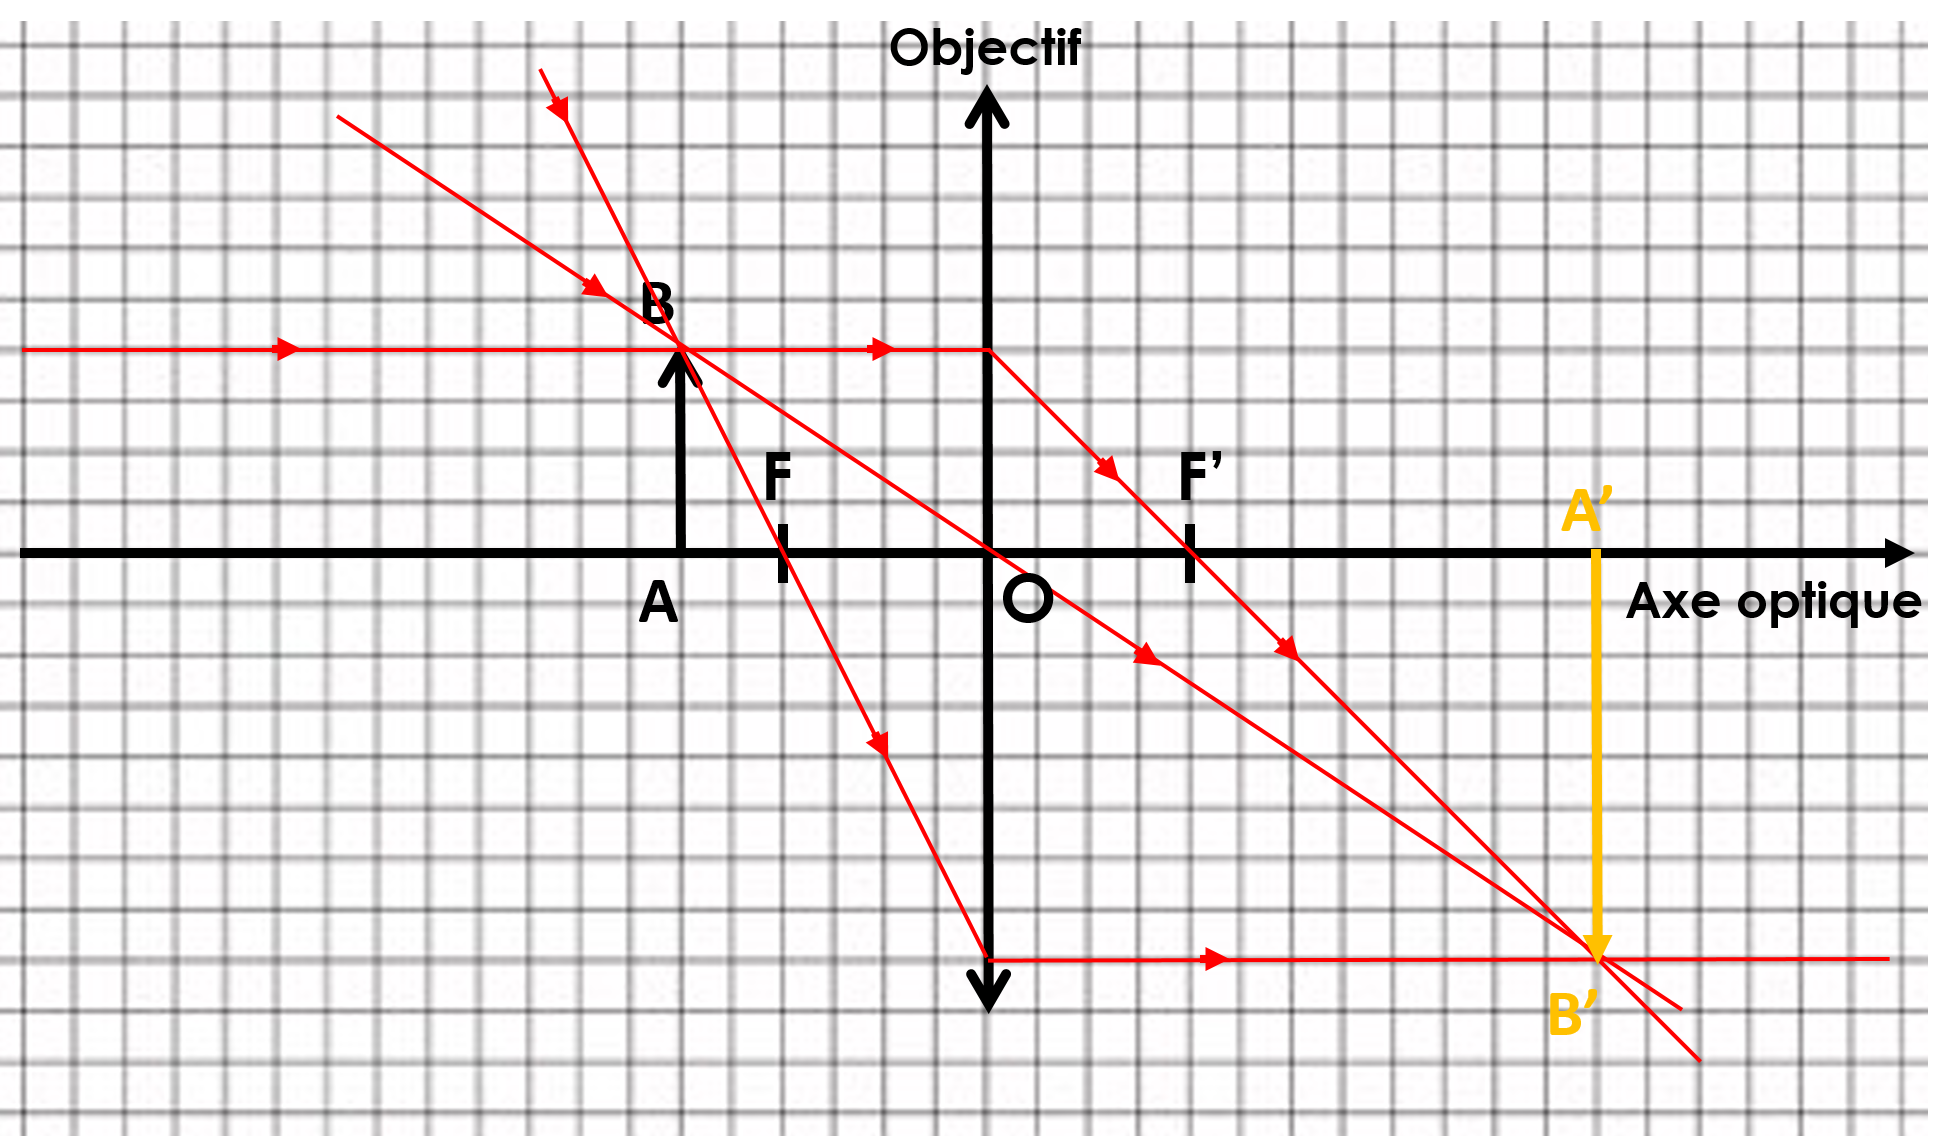
\includegraphics[scale=0.45]{Images/Construction_lentille_SujetB_correction2.png}    
\end{center}}{0}

\question{Caractériser l'image obtenue (agrandie, rétrécie, renversée, droite) et en déduire le signe du grandissement $\gamma$. (2pts)\newline
\texteTrouMultiLignes{~}{2}}{L'image est ici agrandie et renversée. Comme l'image est renversée $\gamma<0$.}{0}
%\\
\question{\`{A} l'aide de votre schéma, déterminer la valeur absolue du grandissement $\abs{\gamma}$ (rappel : $\abs{\gamma}>0$) de cette lentille. (1pt)\newline
\texteTrouMultiLignes{~}{2}}{Par lecture graphique (ou avec une règle mais ici le calcul est simple), on a :
\begin{equation*}
    \abs{\gamma} = \frac{\text{A'B'}}{\text{AB}} =\frac{8\text{ carreaux}}{4 \text{ carreaux}} = 2
\end{equation*}}{0}
%\\
\question{$(*)$Cette valeur est-elle cohérente avec votre schéma ? Justifier. (1pt)\newline
\texteTrouMultiLignes{~}{2}}{Oui cette valeur est cohérente car l'image est agrandie et $\abs{\gamma}>1$.}{0}

%\vspace{-5pt}
%\question{$(*)$Sachant qu'il existe un oculaire et un objectif sur un microscope, expliquer pourquoi un observateur voit une image droite à travers le microscope. (1pt)\newline
%\texteTrouMultiLignes{~}{3}}{L'image à travers une lentille convergente est à chaque fois renversée par rapport à l'objet. Comme l'objet pour l'oculaire est A'B', son image (qu'on peut appeler A"B" par exemple) sera renversée par rapport à A'B'. Elle sera donc dans le même sens que l'objet AB.}{0}
\end{doc}
\clearpage
\begin{doc}{Les essuies-glace automatiques \begin{Large}
    /8 points
\end{Large}}
\setcounter{exercice}{0}
%\begin{wrapfigure}{r}{0.2\textwidth}
\begin{minipage}{0.5\textwidth}
\begin{center}
    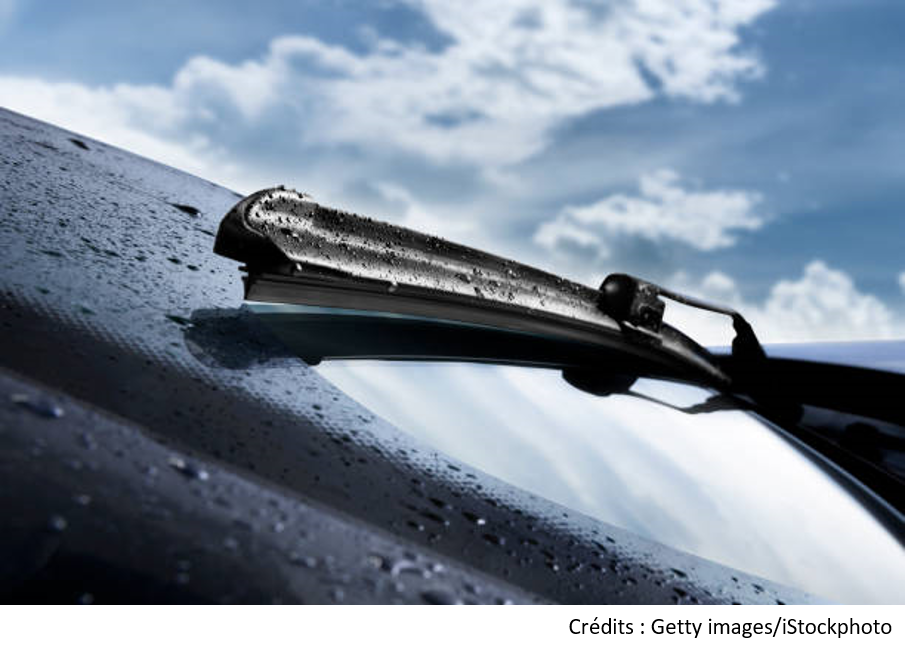
\includegraphics[scale=0.55]{Images/Essuis_glace.png}
\end{center}
\end{minipage}
\begin{minipage}{0.5\textwidth}
\begin{center}
    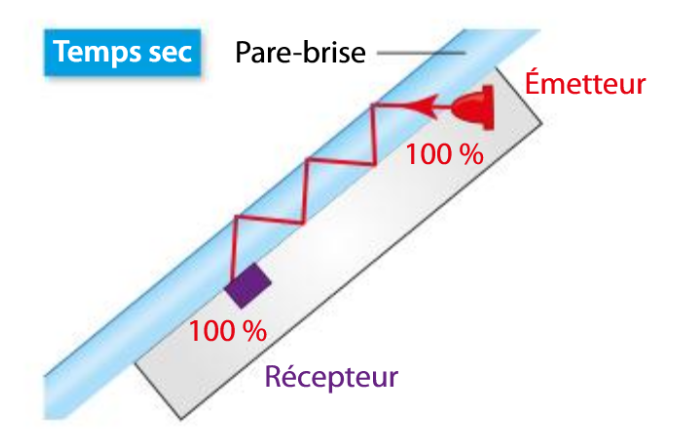
\includegraphics[scale=0.45]{Images/Temps_sec.PNG}
\end{center}
\end{minipage}
Un essuie-glace automatique se met en marche lorsqu'il y a des gouttes de pluie sur le pare-brise. Le schéma ci-dessus illustre le principe de détection d'un faisceau laser envoyé dans un pare-brise (conçu en verre feuilleté) par temps sec : la lumière du laser envoyé par l'émetteur reste confiné dans le pare-brise et arrive jusqu'à un récepteur.\vspace{1cm}%\clearpage

\question{Identifier le phénomène (réflexion, réfraction, dispersion) qui permet au laser de rester confiné dans le pare-brise. (1pt) \newline \texteTrouMultiLignes{~}{1}}{Il s'agit du phénomène de réflexion de la lumière.}{0}
%\\
%\vspace{-0.7cm}
Lorsque la pluie tombe sur le pare-brise, les gouttes d'eau permettent de laisser passer la lumière du laser à l'interface verre-eau. \\
\question{Identifier le phénomène (réflexion, réfraction, dispersion) qui explique la propagation de la lumière du pare-brise vers la goutte d'eau. (1pt)\newline \texteTrouMultiLignes{~}{1}}{Il s'agit du phénomène de réfraction.}{0}
%\\
\vspace{2cm}
Sur la figure de la page suivante, on a réalisé une modélisation de l'interface entre l'essuie-glace (le verre donc) et la goutte d'eau.%\clearpage
\begin{center}
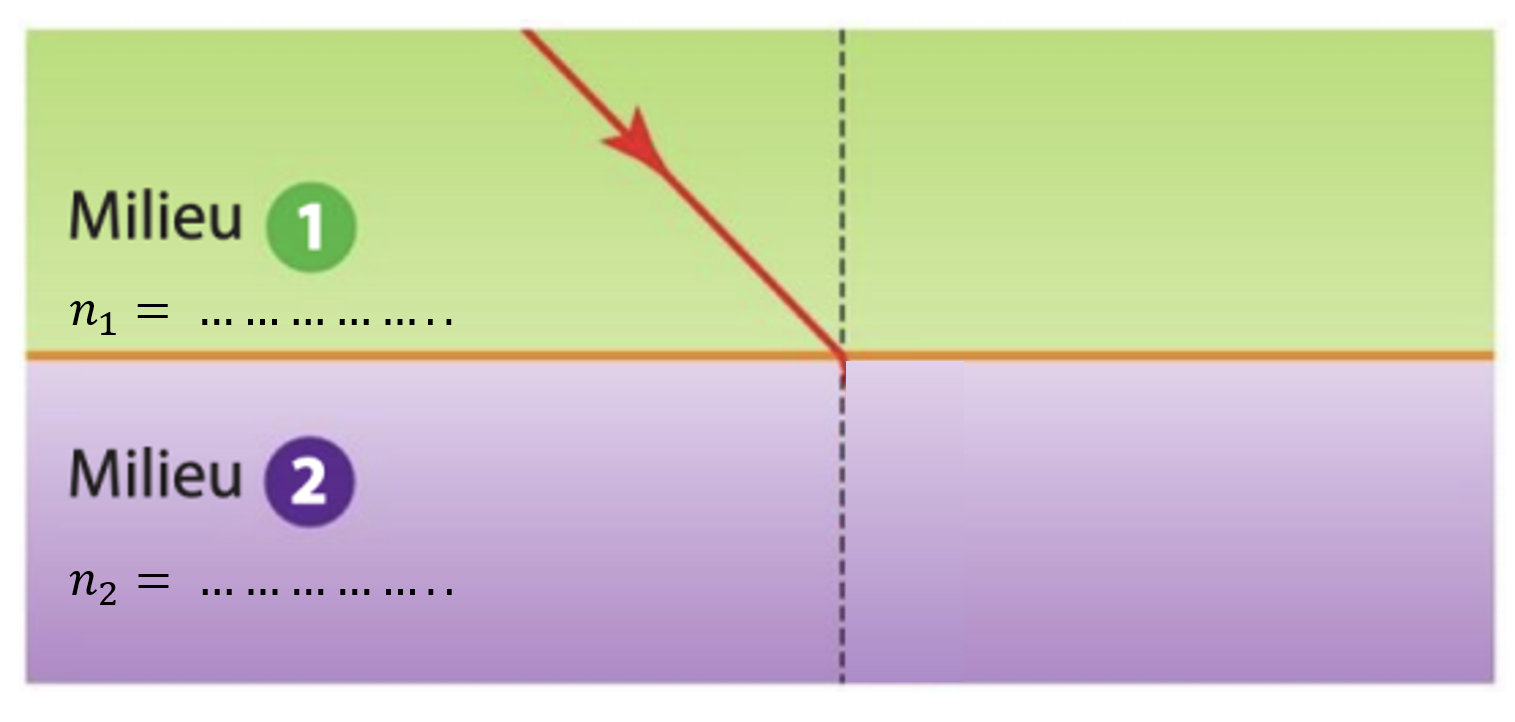
\includegraphics[scale=0.45]{Images/Interface.PNG}    
\end{center}
L'émetteur envoie un rayon lumineux arrivant avec un angle d'incidence $i_1=40\degree$ à cette interface. On donne $n_{\text{eau}}=1,33$ et $n_{\text{verre}}=1,54$.\\
\question{Compléter le schéma en faisant apparaître $n_{verre}$, $n_{eau}$, les rayons incident et réfracté ainsi que le sens de propagation de la lumière, leurs angles associés notés $i_1$ et $i_2$, et enfin la normale au dioptre. (2pts)
}{\begin{center}
    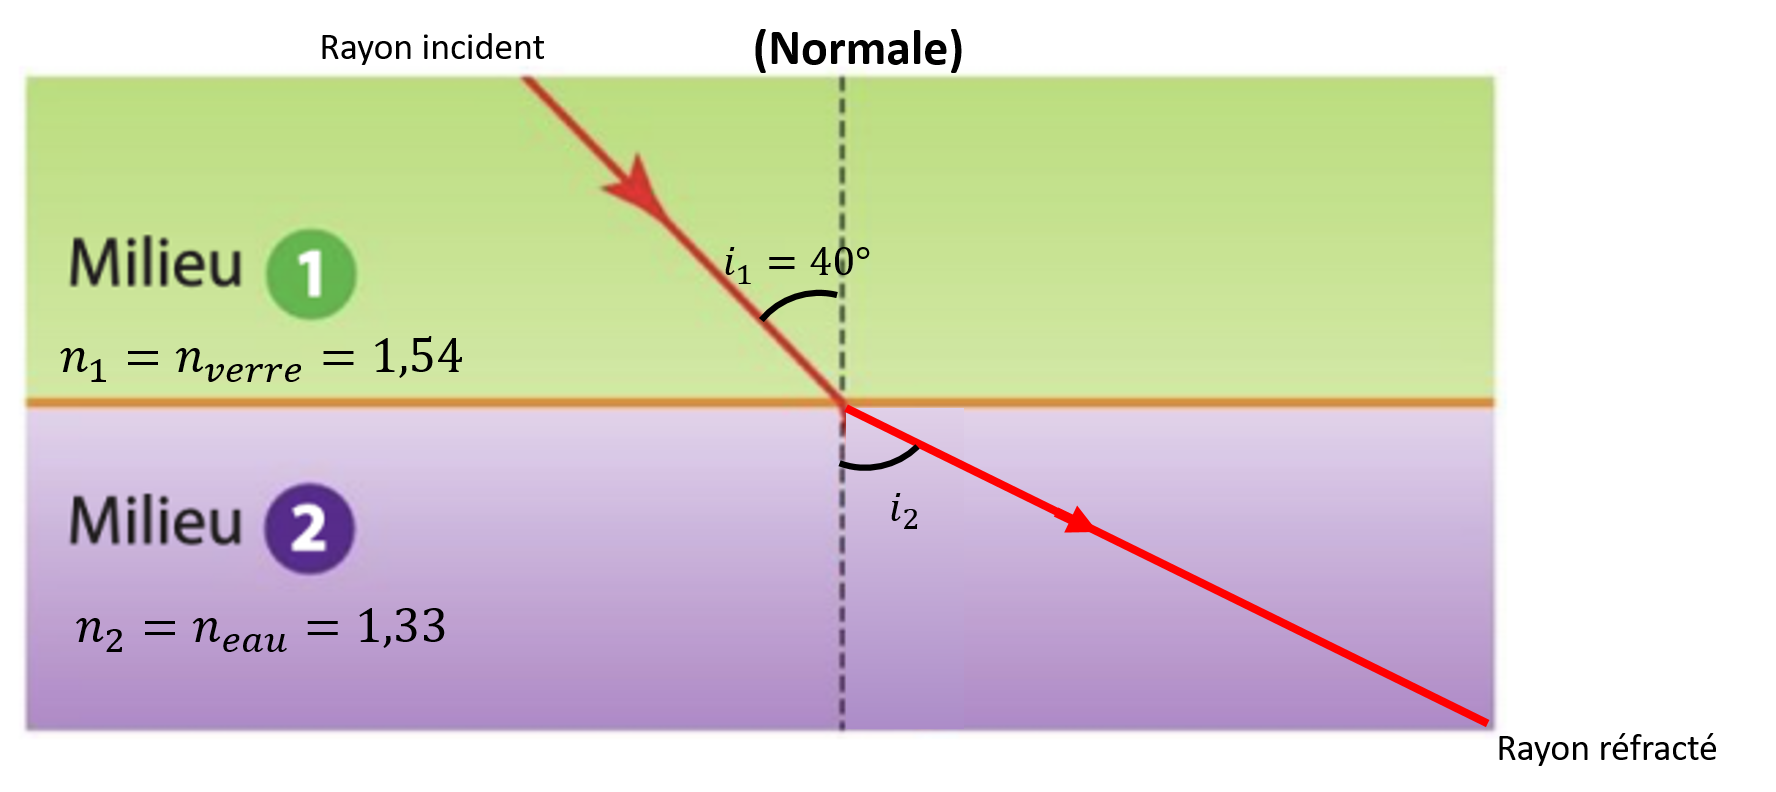
\includegraphics[scale=0.45]{Images/Interface_corriger_sujetB.png}
\end{center}}{0}
%\\
\question{\'{E}noncer la 2$^{\text{ème}}$ loi de Snell-Descartes sur la réfraction. (1pt)\newline
\texteTrouMultiLignes{}{2}}{Le rayon incident, réfracté appartiennent au même plan appelé \textcolor{red}{plan d'incidence}.\\
L'angle d'incidence $i_1$ et l'angle de réfraction $i_2$ sont reliés par la formule suivante :
\begin{empheq}[box=\fbox]{equation*}
    n_1 \sin\left(i_1\right)= n_2 \sin\left(i_2\right)
\end{empheq}}{0}
%\vspace{1cm}
%\\
\question{$(*)$Calculer l'angle de réfraction $i_2$. (2pts)\newline
\texteTrouMultiLignes{~}{3}}{On a d'après la formule précédente : 
\begin{align*}
    n_{\text{verre}} \sin\left(i_1\right)&= n_{\text{eau}} \sin\left(i_2\right) \\
    \text{donc~}\sin\left(i_2\right) &= \frac{n_{\text{verre}}}{n_{\text{eau}}}\sin\left(i_1\right) \\
    \text{donc~} i_2 &= \arcsin\left(\frac{n_{\text{verre}}}{n_{\text{eau}}}\sin\left(i_1\right)\right) = \arcsin\left(\frac{1,54}{1,33}\sin\left(40\degree\right)\right) = 48,1\degree
\end{align*}
La valeur est cohérente car on passe d'un milieu moins réfringeant à un milieu plus réfringeant.}{0}
%\\
Lorsque le récepteur ne reçoit plus 100\% de la lumière émise, les essuies-glace se mettent en marche.\\
\question{$(*)$Expliquer pourquoi les essuies-glace se mettent en route par temps de pluie. (1pt)\newline
\texteTrouMultiLignes{}{3}}{A chaque passage de la lumière à l'interface verre-eau, une partie de la lumière est réfracté et donc sort à l'extérieur du pare-brise. L'intensité diminue donc et le récepteur ne reçoit plus 100\% de la lumière émise déclanchant les essuies-glace.}{0}
%\\
\question{\textit{(Bonus)} Démontrer qu'à partir d'un certain angle d'incidence noté $i_{1,lim}$, il n'y a plus de réfraction. On appelle ce phénomène \textbf{\underline{la réflexion totale}}. (2pts)\newline
\texteTrouMultiLignes{}{4}}{Plus l'angle d'incidence augmente, plus l'angle de réfraction augmente d'après la loi de Descartes sur la réfraction. Comme $n_{verre}>n_{eau}$, $i_1<i_2$. Or comme les angles ne peuvent prendre que des valeurs entre 0 et 90$\degree$, il existe un angle $i_{i,lim}$ à partir duquel $i_{2}=90\degree$. Au-delà de cet angle d'incidence, il n'existe plus de rayon réfracté et toute l'intensité de la lumière est réfléchie dans le pare-brise.}{0}
\end{doc}

\begin{facile}{Bonus de relecture (+0,5pt)}
    Relisez vos réponses et évaluez votre copie sur 20. \\
    \begin{center}
        Selon moi, je pense avoir ...../20
    \end{center}
    Si la différence entre votre note réelle est celle que vous évaluez est supérieure à 2 points, le bonus ne comptera pas.
\end{facile}